\chapter{Introduction}\label{chap:introduction}

\section{Background}

Lambek:
\begin{equation}
\begin{tikzcd}[row sep=1cm, column sep=0.6cm]
& \parbox{1.5cm}{\linespread{-0.5}\selectfont\centering type theory} \arrow[dl,dash,"Curry-","Howard"',sloped] \arrow[dr,dash,"\text{obvious}",sloped] & \\
\mbox{logic} & {} & \parbox{1.5cm}{\linespread{-0.5}\selectfont\centering category theory} \arrow[ll,"\text{internal}"',"\text{language}"]
\end{tikzcd}
\end{equation}

I am very curious to see if the two algebras below would coincide?
\begin{equation}
\begin{tikzcd}[row sep=1cm, column sep=0.6cm]
 & & \parbox{1.5cm}{\linespread{-0.5}\selectfont\centering type theory} \arrow[dl,dash] \arrow[dr,dash] & & & \\
\parbox{2cm}{\linespread{-0.5}\selectfont\centering algebraic logic} \arrow[rrrrr, dashed, dash, bend right,"?"] \arrow[r,dash] & \mbox{logic} \arrow[rr,dash] & {} & \parbox{1.5cm}{\linespread{-0.5}\selectfont\centering category theory} \arrow[r,dash] & \mbox{topos} \arrow[r,dash] & \parbox{2cm}{\linespread{-0.5}\selectfont\centering algebraic geometry}
\end{tikzcd}
\end{equation}

\section{Paul Halmos' algebraic logic}

Every Boolean algebra $\mathbb{A}$ is isomorphic to the set of all continuous functions from $X$ into $\mathbb{O}$, where $X$ is the dual space of the algebra $\mathbb{A}$, and $\mathbb{O}$ is the Boolean algebra with 2 elements.  If there is a homomorphism $f$ between Boolean algebras $\mathbb{A} \rightarrow \mathbb{B}$ then there is a dual morphism $f^*$ between their dual spaces $Y \rightarrow X$:
\begin{equation}
\begin{tikzcd}[column sep=3cm, row sep=0.6cm]
\mathbb{A} \arrow[r,"f"] \arrow[d,shift left=2,phantom,"\cong"{anchor=south,rotate=90}] & \mathbb{B} \arrow[d,shift left=2,phantom,"\cong"{anchor=south,rotate=90}] \\
\overbracket{X} \arrow[d] & \overbracket{Y} \arrow[d] \arrow[l,"f^*"] \\
\underbracket{\mathbb{O}} & \underbracket{\mathbb{O}} 
\end{tikzcd}
\end{equation}

\section{Yuri Manin and Russians}



\section{Topos and internal language}

\section{Term rewriting and all that}



\section{The set-up}

The set of equations $F$ defines an algebraic set = \textbf{the world}:
\begin{equation}
F(x) = 0 .
\end{equation}
The objective of an intelligent agent is to learn $F$.

We have the function $f$ performing \textbf{prediction} of the immediate future:
\begin{equation}
\boxed{\mbox{current state}} \quad x_t \stackrel{f}{\mapsto} x_{t+1} \quad \boxed{\mbox{next state}} \;.
\end{equation}

In an infinitesimal sense, we can see $f$ as a \textbf{differential equation} describing the \textbf{world trajectory}:
\begin{equation}
\dot{x} = f(x) .
\end{equation}
So $F$ is the \textbf{solution} to this differential equation.

It seems that $F$ and $f$ are more or less equivalent ways to describe the world.

Logic can be turned into some form of algebra, and this algebra can be used to express either $F$ or $f$.  Perhaps both ways are feasible, or even mixing the two.

What does it mean to use logic to express $F$ or $f$?

The following table depicts the main correspondences relevant to our research:
\begin{equation}
\begin{tabular}{|c|c|c|}
	\hline
	\textbf{LOGIC} & \textbf{facts} & \textbf{rules} \\
		& \mbox{human(socrates)} & $\forall x. \mbox{human}(x) \rightarrow \mbox{mortal}(x)$ \\
	\hline
	\textbf{ALGEBRA} & \textbf{element} & \textbf{element} \\
		& $p \in \mathbb{A} $ & $(p \rightarrow q) \in \mathbb{A} $ \\
	\hline
	\textbf{WORLD} & \textbf{states} & \textbf{state transitions} \\
		& $x_t$ & $x_t \stackrel{f}{\mapsto} x_{t+1}$ \\
	\hline
\end{tabular}
\end{equation}
The relation between LOGIC and WORLD has been elucidated quite thoroughly in the AI literature.  Note that the state $x_t$ is made up of a set of facts (logic propositions).  A single step of logic inference results in a new conclusion $\delta x$ which is \textit{added} (as a set element) to the current state $x_t$ to form a new state $x_{t+1}$.  Here $t$ refers to ``mental time'' which does not necessarily coincide with real time.

\section{From abstract algebraic logic to concrete computations}

There are two main routes to make abstract algebraic logic concrete:
\begin{itemize}
	\item Find \textbf{matrix representations} of the logical algebra
	\item Implement the logical algebra as the commutative algebra of (classical) \textbf{polynomials}
\end{itemize}

\section{What does it mean to train the AI?}

From the previous section,
\begin{equation}
F(x) = 0 \quad \mbox{is the solution to} \quad \dot{x} = f(x)
\end{equation}
and the two descriptions (by $F$ or by $f$) are equivalent.

The sensory data from the AI are a set of ``world'' points $\{ x_i \}$  and we require either:
\begin{equation}
F(x_t) = 0 \quad \mbox{or} \quad f(x_t) = \delta x = x_{t+1} - x_t
\end{equation}
and $F$ or $f$ can be trained by gradient descent to eliminate errors in the above conditions (equations).

\begin{itemize}
	\item the $x_t$'s are represented as \textbf{logic facts}
	\item $F$ or $f$ is represented as \textbf{logic rules}
\end{itemize}
and we need to \textbf{evaluate} $F(x_t)$ or $f(x_t)$.

Let's do some examples:
\begin{equation}
\begin{tabular}{|c|c|}
	\hline
	\textbf{Logic formula} & \textbf{Algebraic form} \\
	\hline
	human(socrates) & h(s) = 1 \\
	\hline
	human(socrates) $\wedge$ human(plato) & h(s) $\cdot$ h(p) = 1 \\
	\hline
	human(socrates) $\rightarrow$ mortal(socrates) &  1 + h(s) + h(s) $\cdot$ m(s) = 1 \\
	\hline
	$\forall x.$ human($x$) & $h(x)$ is a propositional function \\
		& $\forall_x h(x)$ is a constant function mapping to 1 or 0 \\
	\hline
	$\forall x.$ human($x$) $\rightarrow$ mortal($x$) & $\forall_x \bigl( 1 + h(x) + h(x) \cdot m(x) \bigr) $ \\
		& is a constant function mapping to 1 or 0 \\
	\hline
	$\forall x,y,z.$ father($x,y$) $\wedge$ father($y,z$) $\rightarrow$ & $\forall_x \forall_y \forall_z \bigl( 1 + f(x,y) \cdot f(y,z) + f(x,y) \cdot f(y,z) \cdot g(x,z) \bigr) $ \\
	grandfather($x,z$) & $\mapsto$ 0 or 1 \\
	\hline
	\textbf{general Horn formula}: & $\forall_{x...} \big( 1 + P \cdot Q \cdot R .... + P \cdot Q \cdot R ... \cdot Z \big) $ \\
	$\forall_{x...} P \wedge Q \wedge R ... \rightarrow Z$ & $\mapsto$ 0 or 1 \\
	\hline
\end{tabular}
\nonumber
\end{equation}

Now imagine there are millions of such rules.  Number of predicates obviously increases.

Does each equation require new variables, or can variables be re-used? Seems yes, can be re-used.

The \textbf{loss function} would be the sum of squared errors over all equations:
\begin{equation}
\mathcal{L} = \sum_{\mathrm{eqns}} \epsilon^2 = \sum_i \big( \phi_i (x...) - 1 \big)^2 .
\end{equation}
Learning means to perform the \textbf{gradient descent} via $ \nabla_\Phi \mathcal{L} = \frac{\partial \mathcal{L}}{\partial \Phi} $ where $\Phi$ is the set of parameters for the equations.

How are new conclusions added to the state?  What is the state?  State = set of facts = set of \textbf{grounded} equations.

Inference:  how to get from current state to next state?  Big problem!!  New ground facts have to be read off from satisfaction of all equations.  Rather intractable...

Go back to a physics example:
\begin{equation}
\vcenter{\hbox{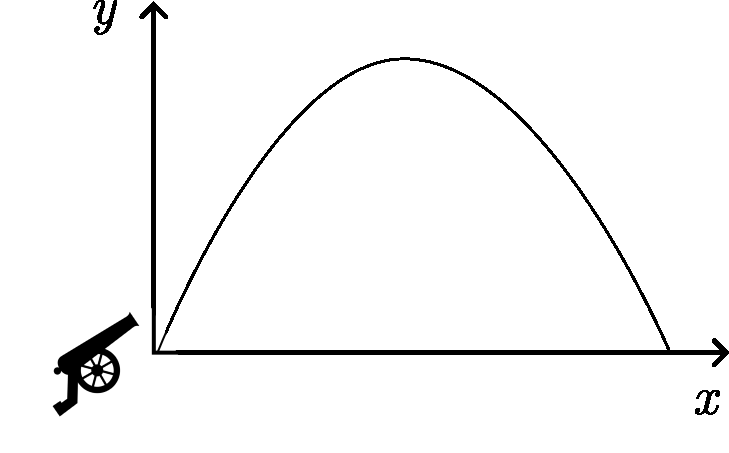
\includegraphics[scale=0.7]{canonball-parabola.png}}}
\end{equation}
The parabola is given by the quadratic equation from high school:
\begin{equation}
	F(x) = 0 \qquad F(x) = ax^2 + bx + c
\end{equation}
but the trajectory can also be described by the physics equation parameterized by time $t$:
\begin{equation}
	\dot{\mathbf{x}} = f(\mathbf{x}) = (v_x, v_y) = (v^0_x , -gt + v^0_y) .
\end{equation}
This parametric form is not unique.  For example, another way is for the point $\mathbf{x}$ to move with uniform speed along the trajectory.

$f(x)$ is the functional form we want, 

Potential problems:
\begin{itemize}
	\item How to represent the set of equations efficiently?  Matrix of coefficients seems wasteful.
	\item We have lost the ``\textbf{deepness}'' of deep learning, but there is recent research showing that \textbf{shallow learning} may work well too.
	\item Need to iterate logical inference multiple times using the same set of equations.
\end{itemize}

